%
% This document is released under the GPL
% Initially written by Stefan Reinauer, <stepan@coresystems.de>
%

\documentclass[titlepage,12pt]{article}
\usepackage{a4}
\usepackage{graphicx}
\usepackage{url}
\usepackage[pdftex]{hyperref}
% \usepackage{makeidx}
% \makeindex

\hypersetup{
	urlbordercolor={1 1 1},
	menubordercolor={1 1 1},
	linkbordercolor={1 1 1},
	colorlinks=false,
	% pdfpagemode=None,  % PDF-Viewer starts without TOC
	% pdfstartview=FitH,
	pdftitle={coreboot on AMD64},
	pdfauthor={Stefan Reinauer},
	pdfsubject={coreboot configuration and build process},
	pdfkeywords={coreboot, Opteron, AMD64, configuration, Build}
}


% \newcommand{\sh}[1]{\begin{verbatim}\texttt{#1}\end{verbatim}}
% \newcommand{\prog}[1]{\textit{#1}}

\setlength{\parindent}{0pt}

\title{coreboot on AMD64}
\author{Stefan Reinauer $<$stepan@coresystems.de$>$}
\date{April 19th, 2009}

\begin{document}

\maketitle

\thispagestyle{empty}

\tableofcontents

\newpage

%
% 1 Abstract
%

\section{Abstract}

This document targets porting coreboot to new mainboards and creating
custom firmware images using coreboot. It describes how to build
coreboot images for the AMD64 platform, including hypertransport
configuration and pertinent utilities. If you are missing information or
find errors in the following descriptions, contact
\href{mailto:stepan@coresystems.de}{\textit{Stefan Reinauer $<$stepan@coresystems.de$>$}}


%
% 2 Changes
%

\section{Changes}
 \begin{itemize}
 \item 2009/04/19 replace LinuxBIOS with coreboot
 \item 2004/06/02 url and language fixes from Ken Fuchs $<$kfuchs@winternet.com$>$
 \item 2004/02/10 acpi and option rom updates
 \item 2003/11/18 initial release
 \end{itemize}



%
% 3 What is coreboot
%

\section{What is coreboot?}

coreboot aims to replace the normal BIOS found on x86, AMD64, PPC,
Alpha, and other machines with a Linux kernel that can boot Linux from a cold
start. The startup code of an average coreboot port is about 500 lines of
assembly and 5000 lines of C. It executes 16 instructions to get into 32bit
protected mode and then performs DRAM and other hardware initializations
required before Linux can take over.

The projects primary motivation initially was maintenance of large
clusters. Not surprisingly interest and contributions have come from
people with varying backgrounds.  Nowadays a large and growing number of
Systems can be booted with coreboot, including embedded systems,
Desktop PCs and Servers.

%
% 4 Build Requirements
%

\section{Build Requirements}
To build coreboot for AMD64 from the sources you need a recent Linux
system for x86 or AMD64. SUSE Linux 8.2 or 9.0 are known to work fine.
The following toolchain is recommended:

 \begin{itemize}
 \item GCC 3.3.1
 \item binutils 2.14.90.0.5
 \item Python 2.3
 \item CVS 1.11.6
 \end{itemize}

\textbf{NOTE:} Later versions should also work. Prior versions might lead to problems.

\newpage

%
% 5 Getting the Sources
%

\section{Getting the Sources}

The latest coreboot sources are available via subversion. The subversion
repository is maintained at SourceForge.net (the project name is
\emph{FreeBIOS}).  First you should create a directory for your
coreboot trees:

{ \small
\begin{verbatim}
$ mkdir coreboot
$ cd coreboot
\end{verbatim}
}

You can get the entire source tree via SVN:

{ \small
\begin{verbatim}
$ svn co svn://coreboot.org/repos/trunk/coreboot-v2
\end{verbatim}
}

Once the source tree is checked out, it can be updated with:

{ \small
\begin{verbatim}
% svn update
\end{verbatim}
}

For the case your corporate firewall blocks port 3690 (subversion) we set up a
snapshot site that keeps the last few hundred source code revisions. It
is available at \url{http://qa.coreboot.org/}.
Due to major structural enhancements to \hbox{coreboot}, AMD64 support
is only available in the \texttt{coreboot-v2} tree. This tree reflects (as
of November 2003) coreboot version 1.1.5 and will lead to coreboot 2.0
when finished.  Most x86 hardware is currently only supported by the
coreboot 1.0 tree.

%
% 6 coreboot configuration overview
%

\section{coreboot configuration overview}
To support a large variety of existing hardware coreboot allows for a
lot of configuration options that can be tweaked in several ways:

\begin{itemize}
\item
Firmware image specific configuration options can be set in the image
configuration file which is usually found in
\texttt{coreboot-v2/targets/$<$vendor$>$/$<$mainboard$>$/}.  Such
options are the default amount of output verbosity during bootup, image
size, use of fallback mechanisms, firmware image size and payloads
(Linux Kernel, Bootloader...) The default configuration file name is
\texttt{Config.lb}, but coreboot allows multiple configurations to
reside in that directory.

\item Mainboard specific configuration options can be set in the
mainboard configuration file placed in
\texttt{coreboot-v2/src/mainboard/$<$vendor$>$/$<$mainboard$>$}. The
mainboard configuration file is always called \texttt{Config.lb}. It
contains information on the onboard components of the mainboard like
CPU type, northbridge, southbridge, hypertransport configuration and
SuperIO configuration.  This configuration file also allows to include
addon code to hook into the coreboot initialization mechanism at
basically any point.

\end{itemize}

This document describes different approaches of changing and configuring the
coreboot source tree when building for AMD64.

%
% 7 Building coreboot
%

\section{Building coreboot}
One of the design goals for building coreboot was to keep object files
out of the source tree in a separate place. This is mandatory for
building parallel coreboot images for several distinct mainboards
and/or platforms. Therefore building coreboot consists of two steps:
\begin{itemize}
\item
creating a build tree which holds all files automatically created by the
configuration utility and the object files
\item
compiling the coreboot code and creating a flashable firmware image.
\end{itemize}

The first of these two steps is accomplished by the \texttt{buildtarget}
script found in \texttt{coreboot-v2/targets/}. To build coreboot for
instance for the AMD Solo Athlon64 mainboard enter:

\begin{verbatim}
% cd coreboot-v2/targets
% ./buildtarget amd/solo
\end{verbatim}

This will create a directory containing a Makefile and other software
components needed for this build. The directory name is defined in the
firmware image specific configuration file. In the case of AMD's Solo
mainboard the default directory resides in
\texttt{coreboot-v2/targets/amd/solo/solo}. To build the coreboot image, do

\begin{verbatim}
% cd amd/solo/solo
% make
\end{verbatim}

The coreboot image filename is specified in the firmware image specific
configuration file. The default filename for AMD's Solo mainboard is
\texttt{solo.rom}.

%
% 8 Programming coreboot to flash memory
%

\section{Programming coreboot to flash memory}
The image resulting from a coreboot build can be directly programmed to
a flash device, either using a hardware flash programmer or by using the
Linux flash driver devbios or mtd. This document assumes that you use a
hardware flash programmer. If you are interested in doing in-system
software flash programming, find detailed information:

\begin{itemize}
\item \url{http://www.openbios.org/development/devbios.html} (/dev/bios)
\item \url{http://www.linux-mtd.infradead.org/} (Memory Technology Device Subsystem MTD)
\end{itemize}

\newpage

%
% 9 coreboot configuration
%

\section{coreboot configuration}
The following chapters will cope with configuring coreboot. All
configuration files share some basic rules
\begin{itemize}
\item
The default configuration file name in coreboot is \texttt{Config.lb}.
\item
All variables used in a configuration file have to be declared in this
file with \texttt{uses VARNAME} before usage.
\item
Comments can be added on a new line by using the comment identifier
\texttt{\#} at the beginning of the line.
\item
coreboot distinguishes between statements and options. Statements cause
the coreboot configuration mechanism to act, whereas options set
variables that are used by the build scripts or source code.
\item
Default configuration values can be set in the mainboard configuration
files (keyword default)
\item
Option overrides to the default configuration can only be specified in
the build target configuration file
\texttt{coreboot-v2/targets/$<$vendor$>$/$<$mainboard$>$/Config.lb}
(keyword option)
\end{itemize}

\subsection{Common Configuration Statements}

\begin{itemize}

\item \begin{verbatim}uses\end{verbatim}

All local configuration variables have to be declared before they can be
used. Example:
\begin{verbatim}
        uses CONFIG_ROM_IMAGE_SIZE
\end{verbatim}

\textbf{NOTE:} Only configuration variables known to the configuration
system can be used in configuration files. coreboot checks
\texttt{coreboot-v2/src/config/Options.lb} to see whether a configuration
variable is known.

\item \begin{verbatim}default\end{verbatim}

The \texttt{default} statement is used to set a configuration variable
with an overridable default value. It is commonly used in mainboard
configuration files.

Example:

\begin{verbatim}
        default CONFIG_ROM_IMAGE_SIZE=0x10000
\end{verbatim}

It is also possible to assign the value of one configuration variable to
another one, i.e.:

\begin{verbatim}
        default CONFIG_FALLBACK_SIZE=CONFIG_ROM_SIZE
\end{verbatim}

Also, simple expressions are allowed:

\begin{verbatim}
        default CONFIG_FALLBACK_SIZE=(CONFIG_ROM_SIZE -  NORMAL_SIZE)
\end{verbatim}

If an option contains a string, this string has to be protected with
quotation marks:

\begin{verbatim}
        default CC="gcc -m32"
\end{verbatim}

\item \begin{verbatim}option\end{verbatim}

The \texttt{option} statement basically behaves identically to the
\texttt{default} statement. But unlike default it can only be used in
build target configuration files
(\texttt{coreboot-v2/targets/$<$vendor$>$/$<$mainboard$>$}). The option
statement allows either to set new options or to override default values
set with the default statement in a mainboard configuration file.
Syntax and application are the same as with default.

\end{itemize}

\subsection{Firmware image specific configuration}
coreboot allows to create different firmware images for the same
hardware. Such images can differ in the amount of output they produce,
the payload, the number of subimages they consist of etc.

The firmware image specific configuration file can be found in \\
\texttt{coreboot-v2/targets/$<$vendor$>$/<mainboard$>$}.

\subsubsection{Firmware image specific keywords}
In addition to the above described keywords the following statements are
available in firmware image specific configuration files:

\begin{itemize}
\item \begin{verbatim}romimage\end{verbatim}

The \texttt{romimage} definition describes a single rom build within the
final coreboot image. Normally there are two romimage definitions per
coreboot build: \texttt{normal} and \texttt{fallback}.

Each \texttt{romimage} section needs to specify a mainboard directory and a
payload. The mainboard directory contains the mainboard specific
configuration file and source code. It is specified relatively to
\texttt{coreboot-v2/src/mainboard}. The payload definition is an absolute
path to a static elf binary (i.e Linux kernel or etherboot)

\begin{verbatim}
romimage "normal"
        option CONFIG_USE_FALLBACK_IMAGE=0
        option CONFIG_ROM_IMAGE_SIZE=0x10000
        option COREBOOT_EXTRA_VERSION=".0Normal"
        mainboard amd/solo
        payload /suse/stepan/tg3ide_
        disk.zelf
end
\end{verbatim}

\item \begin{verbatim}buildrom\end{verbatim}

The \texttt{buildrom} statement is used to determine which of the
coreboot image builds (created using \texttt{romimage}) are packed
together to the final coreboot image. It also specifies the order of
the images and the final image size:

\begin{verbatim}
        buildrom ./solo.rom CONFIG_ROM_SIZE "normal" "fallback"
\end{verbatim}

\end{itemize}


\subsubsection{Firmware image configuration options}
In addition to the definitions described above there are a number of
commonly used options. Configuration options set in the firmware image
specific configuration file can override default selections from the
Mainboard specific configuration.  See above examples about
option on how to set them.

\begin{itemize}

\item \begin{verbatim}CC\end{verbatim}

Target C Compiler. Default is \texttt{\$(CROSS\_COMPILE)gcc}. Set to
\texttt{gcc -m32} for compiling AMD64 coreboot images on an AMD64
machine.

\item \begin{verbatim}CONFIG_CHIP_CONFIGURE \end{verbatim}

Use new \textit{chip\_configure} method for configuring (nonpci)
devices. Set to \texttt{1} for all AMD64 mainboards.

\item \begin{verbatim}CONFIG_DEFAULT_CONSOLE_LOGLEVEL\end{verbatim}

Console will log at this level unless changed. Default is \texttt{7},
minimum is \texttt{0}, maximum is \texttt{10}.

\item \begin{verbatim}CONFIG_CONSOLE_SERIAL8250\end{verbatim}

Log messages to 8250 uart based serial console. Default is \texttt{0}
(don't log to serial console). This value should be set to \texttt{1}
for all AMD64 builds.

\item \begin{verbatim}CONFIG_ROM_SIZE\end{verbatim}

Size of final ROM image. This option has no default value.

\item \begin{verbatim}CONFIG_FALLBACK_SIZE\end{verbatim}

Fallback image size. Defaults to \texttt{65536} bytes. \textbf{NOTE:}
This does not include the fallback payload.

\item \begin{verbatim}CONFIG_HAVE_OPTION_TABLE\end{verbatim}

Export CMOS option table. Default is \texttt{0}. Set to \texttt{1} if
your mainboard has CMOS memory and you want to use it to store
coreboot parameters (Loglevel, serial line speed, ...)

\item \begin{verbatim}CONFIG_ROM_PAYLOAD\end{verbatim}

Boot image is located in ROM (as opposed to \texttt{CONFIG\_IDE\_PAYLOAD}, which
will boot from an IDE disk)

\item \begin{verbatim}CONFIG_HAVE_FALLBACK_BOOT\end{verbatim}

Set to \texttt{1} if fallback booting is required. Defaults to
\texttt{0}.

\end{itemize}


The following options should be used within a romimage section:

\begin{itemize}

\item \begin{verbatim}CONFIG_USE_FALLBACK_IMAGE\end{verbatim}

Set to \texttt{1} to build a fallback image. Defaults to \texttt{0}

\item \begin{verbatim}CONFIG_ROM_IMAGE_SIZE\end{verbatim}

Default image size. Defaults to \texttt{65535} bytes.

\item \begin{verbatim}COREBOOT_EXTRA_VERSION\end{verbatim}

coreboot extra version. This option has an empty string as default. Set
to any string to add an extra version string to your coreboot build.

\end{itemize}

\newpage

\subsection{Mainboard specific configuration}

Mainboard specific configuration files describe the onboard
mainboard components, i.e. bridges, number and type of CPUs. They also
contain rules for building the low level start code which is translated
using romcc and/or the GNU assembler.  This code enables caches and
registers, early mtrr settings, fallback mechanisms, dram init and
possibly more.

\textbf{NOTE:} The \texttt{option} keyword can not be used in mainboard
specific configuration files.  Options shall instead be set using the
\texttt{default} keyword so that they can be overridden by the image
specific configuration files if needed.

\subsubsection{Mainboard specific keywords}

The following statements are used in mainboard specific configuration
files:

\begin{itemize}
\item \begin{verbatim}arch\end{verbatim}

Sets the CPU architecture. This should be \texttt{i386} for AMD64 boards.\\
Example:

\begin{verbatim}
        arch i386 end
\end{verbatim}

\item \begin{verbatim}cpu\end{verbatim}

The cpu statement is needed once per possibly available CPU. In a
one-node system, write:

\begin{verbatim}
        cpu k8 "cpu0" end
\end{verbatim}

\item \begin{verbatim}driver\end{verbatim}

The \texttt{driver} keyword adds an object file to the driver section of a
coreboot image.  This means it can be used by the PCI device
initialization code. Example:

\begin{verbatim}
        driver mainboard.o
\end{verbatim}

\item \begin{verbatim}object\end{verbatim}

The \texttt{object} keyword adds an object file to the coreboot image.
Per default the object file will be compiled from a \texttt{.c} file
with the same name. Symbols defined in such an object file can be used
in other object files and drivers. Example:

\begin{verbatim}
        object reset.o
\end{verbatim}

\item \begin{verbatim}makerule\end{verbatim}

This keyword can be used to extend the existing file creation rules
during the build process. This is useful if external utilities have to
be used for the build. coreboot on AMD64 uses romcc for it's early
startup code placed in auto.c.

To tell the configuration mechanism how to build \texttt{romcc} files,
do:

\begin{verbatim}
makerule ./auto.E
        depends "$(CONFIG_MAINBOARD)/auto.c option_table.h ./romcc"
        action "./romcc -E -mcpu=k8 -O2 -I$(TOP)/src -I. $(CPPFLAGS) \
		$(CONFIG_MAINBOARD)/auto.c -o $@"
end
makerule ./auto.inc
        depends "$(CONFIG_MAINBOARD)/auto.c option_table.h ./romcc"
        action "./romcc    -mcpu=k8 -O2 -I$(TOP)/src -I. $(CPPFLAGS) \
                $(CONFIG_MAINBOARD)/auto.c -o $@"
end
\end{verbatim}

Each \texttt{makerule} section contains file dependencies (using the
texttt{depends} keyword) and an action that is taken when the dependencies
are satisfied (using the \texttt{action} keyword).

\item \begin{verbatim}mainboardinit\end{verbatim}

With the mainboardinit keyword it's possible to include assembler code
directly into the coreboot image. This is used for early infrastructure
initialization, i.e. to switch to protected mode. Example:

\begin{verbatim}
        mainboardinit cpu/i386/entry16.inc
\end{verbatim}

\item \begin{verbatim}ldscript\end{verbatim}

The GNU linker ld is used to link object files together to a coreboot
ROM image.

Since it is a lot more comfortable and flexible to use the GNU linker
with linker scripts (ldscripts) than to create complex command line
calls, coreboot features including linker scripts to control image
creation. Example:

\begin{verbatim}
        ldscript /cpu/i386/entry16.lds
\end{verbatim}


\item \begin{verbatim}dir\end{verbatim}

coreboot reuses as much code between the different ports as possible.
To achieve this, commonly used code can be stored in a separate
directory. For a new mainboard, it is enough to know that the code in
that directory can be used as is.

coreboot will also read a \texttt{Config.lb} file stored in that
directory. This happens with:

\begin{verbatim}
        dir /pc80
\end{verbatim}


\item \begin{verbatim}config\end{verbatim}

This keyword is needed by the new chip configuration scheme. Should be
used as:

\begin{verbatim}
        config chip.h
\end{verbatim}

\item \begin{verbatim}register\end{verbatim}
The \texttt{register} keyword can occur in any section, passing
additional \\
parameters to the code handling the associated device.
Example:

\begin{verbatim}
        register "com1" = "{1, 0, 0x3f8, 4}"
\end{verbatim}

\item \begin{verbatim}northbridge\end{verbatim}

The \texttt{northbridge} keyword describes a system northbridge. Some
systems, like AMD64, can have more than one northbridge, i.e. one per
CPU node. Each northbridge is described by the path to the northbridge
code in coreboot (relative to \texttt{coreboot-v2/src/northbridge}), i.e.
\texttt{amd/amdk8} and a unique name (i.e \texttt{mc0}) \\
Example:

\begin{verbatim}
        northbridge amd/amdk8 "mc0"
                [..]
        end
\end{verbatim}

\item \begin{verbatim}southbridge\end{verbatim}

To simplify the handling of bus bridges in a coreboot system, all
bridges available in a system that are not northbridges (i.e AGP, IO,
PCIX) are seen as southbridges.

Since from the CPUs point of view any southbridge is connected via the
northbridge, a southbridge section is declared within the northbridge
section of the north bridge it is attached to.

Like the northbridge, any other bridge is described by the path to it's
driver code, and a unique name. If the described bridge is a
hypertransport device, the northbridge's hypertransport link it connects
to can be specified using the \texttt{link} keyword. Example:

\begin{verbatim}
northbridge amd/amdk8 "mc0"
        [..]
        southbridge amd/amd8111 "amd8111" link 0
                [..]
        end
        [..]
end
\end{verbatim}

\item \begin{verbatim}pci\end{verbatim}

The \texttt{pci} keyword can only occur within a \texttt{northbridge} or
\texttt{southbridge} section. It is used to describe the PCI devices
that are provided by the bridge.  Generally all bridge sections have a
couple of \texttt{pci} keywords.

The first occurrence of the \texttt{pci} keyword tells coreboot where
the bridge devices start, relative to the PCI configuration space used
by the bridge. The following occurences of the \texttt{pci} keyword
describe the provided devices.

Adding the option \texttt{on} or \texttt{off} to a PCI device will
enable or disable this device. This feature can be used if some bridge
devices are not wired to hardware outputs and thus are not used.

Example:

\begin{verbatim}
northbridge amd/amdk8 "mc1"
        pci 0:19.0
        pci 0:19.0
        pci 0:19.0
        pci 0:19.1
        pci 0:19.2
        pci 0:19.3
end
\end{verbatim}

or

\begin{verbatim}
southbridge amd/amd8111 "amd8111" link 0
        pci 0:0.0
        pci 0:1.0 on
        pci 0:1.1 on
        pci 0:1.2 on
        pci 0:1.3 on
        pci 0:1.5 off
        pci 0:1.6 off
        pci 1:0.0 on
        pci 1:0.1 on
        pci 1:0.2 on
        pci 1:1.0 off
        [..]
end
\end{verbatim}

\item \begin{verbatim}superio\end{verbatim}

SuperIO devices are basically handled like brigdes. They are taking
their driver code from \texttt{coreboot-v2/src/superio/}. They don't
provide a PCI compatible configuration interface, but instead are ISA
PnP devices. Normally they are connected to a southbridge. If this is
the case, the \texttt{superio} section will be a subsection of the
\texttt{southbridge} section of the southbridge it is connected to.
Example:

\begin{verbatim}
superio nsc/pc87360 link 1
        pnp 2e.0
        pnp 2e.1
        pnp 2e.2
        pnp 2e.3
        pnp 2e.4
        pnp 2e.5
        pnp 2e.6
        pnp 2e.7
        pnp 2e.8
        pnp 2e.9
        pnp 2e.a
        register "com1" = "{1, 0, 0x3f8, 4}"
        register "lpt" = "{1}"
end
\end{verbatim}

\end{itemize}

\newpage

\subsubsection{Mainboard specific configuration options}

The following options are commonly used in mainboard specific
configuration files.

They should be set using the \texttt{default} keyword:

\begin{itemize}

\item \begin{verbatim}CONFIG_HAVE_HARD_RESET\end{verbatim}

If set to \texttt{1}, this option defines that there is a hard reset
function for this mainboard.  This option is not defined per default.

\item \begin{verbatim}CONFIG_HAVE_PIRQ_TABLE\end{verbatim}

If set to \texttt{1}, this option defines that there is an IRQ Table for
this mainboard. This option is not defined per default.

\item \begin{verbatim}CONFIG_IRQ_SLOT_COUNT\end{verbatim}

Number of IRQ slots. This option is not defined per default.

\item \begin{verbatim}CONFIG_HAVE_MP_TABLE\end{verbatim}

Define this option to build an MP table (v1.4). The default is not to
build an MP table.

\item \begin{verbatim}CONFIG_HAVE_OPTION_TABLE\end{verbatim}

Define this option to export a CMOS option table. The default is not to
export a CMOS option table.

\item \begin{verbatim}CONFIG_SMP\end{verbatim}

Set this option to \texttt{1} if the mainboard supports symmetric
multiprocessing (SMP). This option defaults to \texttt{0} (no SMP).

\item \begin{verbatim}CONFIG_MAX_CPUS\end{verbatim}

If \begin{verbatim}CONFIG_SMP\end{verbatim} is set, this option defines
the maximum number of CPUs (i.e. the number of CPU sockets) in the
system. Defaults to \texttt{1}.

\item \begin{verbatim}CONFIG_IOAPIC\end{verbatim}

Set this option to \texttt{1} to enable IOAPIC support. This is
mandatory if you want to boot a 64bit Linux kernel on an AMD64 system.

\item \begin{verbatim}CONFIG_STACK_SIZE\end{verbatim}

coreboot stack size. The size of the function call stack defaults to
\texttt{0x2000} (8k).

\item \begin{verbatim}CONFIG_HEAP_SIZE\end{verbatim}

coreboot heap size. The heap is used when coreboot allocates memory
with malloc(). The default heap size is \texttt{0x2000}, but AMD64 boards
generally set it to \texttt{0x4000} (16k)

\item \begin{verbatim}CONFIG_XIP_ROM_BASE\end{verbatim}

Start address of area to cache during coreboot execution directly from
ROM.

\item \begin{verbatim}CONFIG_XIP_ROM_SIZE\end{verbatim}

Size of area to cache during coreboot execution directly from ROM

\item \begin{verbatim}CONFIG_COMPRESS\end{verbatim}

Set this option to \texttt{1} for a compressed image. If set to
\texttt{0}, the image is bigger but will start slightly faster (since no
decompression is needed).

\end{itemize}


\newpage

%
% 10. Tweaking the source code
%

\section{Tweaking the source code}
Besides configuring the existing code it is sometimes necessary or
desirable to tweak certain parts of coreboot by direct changes to the
code. This chapter covers some possible enhancements and changes that
are needed when porting coreboot to a new mainboard or just come
handy now and then.

\subsection{Hypertransport configuration}
Before coreboot is able to activate all CPUs and detect bridges
attached to these CPUs (and thus, see all devices attached to the
system) it has to initialize the coherent hypertransport devices.

The current algorithms to do coherent hypertransport initialization are
not fully, automatically evaluating the hypertransport chain graph.
Therefore the code needs to be adapted when porting coreboot to a new
AMD64 mainboard. An example arrangement of hypertransport devices
looks like this:

\begin{figure}[htb]
\centering
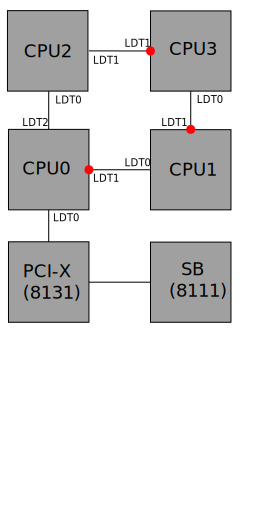
\includegraphics[scale=1.0]{hypertransport.pdf}
\caption{Example: Hypertransport Link Connections}
\label{fix:hypertransport}
\end{figure}

Each hypertransport device has one to three hypertransport links that
are used for device interconnection. These links are called LDT$[$012$]$, or
accordingly UP, ACROSS, DOWN.  Communication between the hypertransport
devices can be freely routed, honoring the physical wiring. Teaching the
coherent hypertransport initialization algorithm this wiring happens in
two steps.

\newpage

\begin{enumerate}
\item Setting outgoing connections
The algorithm needs to know which outgoing port of a CPU node is
connected to the directly succeeding node. This is done in
\texttt{coreboot-v2/src/mainboard/$<$vendor$>$/$<$mainboard$>$/auto.c}
with a number of preprocessor defines (one define for two-node systems,
three defines for four-node systems).

The ports in question are flagged with a circle in the graph for
illustration. For the example graph above (all outgoing connections are
realized using LDT1/ACROSS) the defines are:

\begin{verbatim}
#define CONNECTION_0_1 ACROSS
#define CONNECTION_0_2 ACROSS
#define CONNECTION_1_3 ACROSS
\end{verbatim}

\item Describing routing information between CPUs.

There are basically three different message types for hypertransport
communication:
\begin{enumerate}
\item request packages
\item response packages
\item broadcast packages
\end{enumerate}

These three message types are routed using different hypertransport
ports. The routing information is written to the AMD K8 routing table.
In an Nnode system this routing table consists of 3*N*N entries , one
for each message type and for each possible CPU --> CPU communication. For
simplicity coreboot keeps the 3 routing entries for each CPU --> CPU
communication in one machine word.  The routing table of each node looks
like this:

\begin{verbatim}
/* Routing Table for Node i
 *
 * F0: 0x40, 0x44, 0x48, 0x4c, 0x50, 0x54, 0x58, 0x5c
 * i: 0, 1, 2, 3, 4, 5, 6, 7
 *
 * [ 0: 3] Request Route
 * [0] Route to this node
 * [1] Route to Link 0
 * [2] Route to Link 1
 * [3] Route to Link 2
 * [11: 8] Response Route
 * [0] Route to this node
 * [1] Route to Link 0
 * [2] Route to Link 1
 * [3] Route to Link 2
 * [19:16] Broadcast route
 * [0] Route to this node
 * [1] Route to Link 0
 * [2] Route to Link 1
 * [3] Route to Link 2
 */
\end{verbatim}

The routing table is passed to the coherent hypertransport
initialization algorithm by defining a function called
\texttt{generate\_row()} in \texttt{auto.c}:

\begin{verbatim}
static unsigned int generate_row
                (uint8_t node, uint8_t row, uint8_t maxnodes)
\end{verbatim}

This function is trivial if there is only one CPU in the system, since
no routing has to be done:

\begin{verbatim}
static unsigned int generate_row
                (uint8_t node, uint8_t row, uint8_t maxnodes)
{
        return 0x00010101; /* default row entry */
}
\end{verbatim}

On a two-node system things look slightly more complicated. Since the
coherent hypertransport initialization algorithm works by consecutively
enabling CPUs, it contains routing information for driving the system
with one node and two nodes:

\begin{verbatim}
static unsigned int generate_row
                (uint8_t node, uint8_t row, uint8_t maxnodes)
{
        uint32_t ret=0x00010101; /* default row entry */
        static const unsigned int rows_2p[2][2] = {
                { 0x00050101, 0x00010404 },
                { 0x00010404, 0x00050101 }
        };
        if(maxnodes>2) maxnodes=2;
        if (!(node>=maxnodes || row>=maxnodes)) {
                ret=rows_2p[node][row];
        }
        return ret;
}
\end{verbatim}

Systems with four nodes have to contain routing information for one, two
and four-node setups:

\begin{verbatim}
static unsigned int generate_row
                (uint8_t node, uint8_t row, uint8_t maxnodes)
{
        uint32_t ret=0x00010101; /* default row entry */
        static const unsigned int rows_2p[2][2] = {
                { 0x00030101, 0x00010202 },
                { 0x00010202, 0x00030101 }
        };
        static const unsigned int rows_4p[4][4] = {
                { 0x00070101, 0x00010202, 0x00030404, 0x00010204 },
                { 0x00010202, 0x000b0101, 0x00010208, 0x00030808 },
                { 0x00030808, 0x00010208, 0x000b0101, 0x00010202 },
                { 0x00010204, 0x00030404, 0x00010202, 0x00070101 }
        };
        if (!(node>=maxnodes || row>=maxnodes)) {
                if (maxnodes==2)
                        ret=rows_2p[node][row];
                if (maxnodes==4)
                        ret=rows_4p[node][row];
        }
        return ret;
}
\end{verbatim}
\end{enumerate}

\subsection{DRAM configuration}
Setting up the RAM controller(s) is probably the most complex part of
coreboot.  Basically coreboot serially initializes all RAM controllers
in the system, using SPDROM (serial presence detect) data to set
timings, size and other properties.  The SPD data is usually read
utilizing the I2C SMBUS interface of the southbridge.

There is one central data structure that describes the RAM controllers
available on an AMD64 system and the associated devices:

\begin{verbatim}
struct mem_controller {
        unsigned node_id;
        device_t f0, f1, f2, f3;
        uint8_t channel0[4];
        uint8_t channel1[4];
};
\end{verbatim}

Available mainboard implementations and CPUs create the need to add
special setup code to RAM initialization in a number of places.
coreboot provides hooks to easily add code in these places without
having to change the generic code.  Whether these hooks have to be used
depends on the mainboard design. In many cases the functions executed
by the hooks just carry out trivial default settings or they are even
empty.

Some mainboard/CPU combinations need to trigger an additional memory
controller reset before the memory can be initialized properly. This is,
for example, used to get memory working on preC stepping AMD64
processors. coreboot provides two hooks for triggering onboard memory
reset logic:

\begin{itemize}
\item \begin{verbatim}static void memreset_setup(void)\end{verbatim}
\item \begin{verbatim}static void memreset(int controllers, const struct
		mem_controller *ctrl)\end{verbatim}
\end{itemize}

Some mainboards utilize an SMBUS hub or possibly other mechanisms to
allow using a large number of SPDROMs and thus ram sockets. The result
is that only the SPDROM information of one cpu node is visible at a
time. The following function, defined in \texttt{auto.c}, is called every time
before a memory controller is initialized and gets the memory controller
information of the next controller as a parameter:

\begin{verbatim}
static inline void activate_spd_rom (const struct mem_controller *ctrl)
\end{verbatim}

The way SMBUS hub information is coded into the \texttt{mem\_controller}
structure is mainboard implementation specific and not
described here.  See \texttt{coreboot-v2/src/mainboard/amd/quartet/auto.c}
for an example.

coreboot folks have agreed on SPD data being the central information
source for RAM specific information. But not all mainboards/RAM
modules feature a physical SPD ROM. To still allow an easy to use SPD
driven setup, there is a hook that abstracts reading the SPD ROM
ingredients that are used by the memory initialization mechanism:

\begin{verbatim}
static inline int spd_read_byte(unsigned device, unsigned address)
\end{verbatim}

This function, defined in \texttt{auto.c}, directly maps it's calls to
\texttt{smbus\_read\_byte()} calls if SPD ROM information is read via
the I2C SMBUS:

\begin{verbatim}
static inline int spd_read_byte(unsigned device, unsigned address)
{
        return smbus_read_byte(device & 0xff, address);
}
\end{verbatim}

If there is no SPD ROM available in the system design, this function
keeps an array of SPD ROM information hard coded per logical RAM module.
It returns the faked' SPD ROM information using device and address
as indices to this array.


\subsection {IRQ Tables}

Mainboards that provide an IRQ table should have the following two
variables set in their \texttt{Config.lb} file:

\begin{verbatim}
default CONFIG_HAVE_PIRQ_TABLE=1
default CONFIG_IRQ_SLOT_COUNT=7
\end{verbatim}

This will make coreboot look for the file \\
\texttt{coreboot-v2/src/mainboard/<vendor>/<mainboard>/irq\_tables.c} which
contains the source code definition of the IRQ table. coreboot corrects
small inconsistencies in the IRQ table during startup (checksum and
number of entries), but it is not yet writing IRQ tables in a completely
dynamic way.

\textbf{NOTE:} To get Linux to understand and actually use the IRQ
table, it is not always a good idea to specify the vendor and device id
of the actually present interrupt router device. Linux 2.4 for example
does not know about the interrupt router of the AMD8111 southbridge. In
such cases it is advised to choose the vendor/device id of a compatible
device that is supported by the Linux kernel. In case of the AMD8111
interrupt router it is advised to specify the AMD768/Opus interrupt
controller instead (vendor id=\texttt{0x1022}, device id=\texttt{0x7443})

\subsection {MP Tables}

coreboot contains code to create MP tables conforming the
Multiprocessor Specification V1.4. To include an MP Table in a coreboot
image, the following configuration variables have to be set (in the
mainboard specific configuration file
\texttt{coreboot-v2/src/mainboard/<vendor><mainboard>/Config.lb}):

\begin{verbatim}
default CONFIG_SMP=1
default CONFIG_MAX_CPUS=1 # 2,4,..
default CONFIG_HAVE_MP_TABLE=1
\end{verbatim}

coreboot will then look for a function for setting up the MP table in
the file \texttt{coreboot-v2/src/mainboard<vendor>/<mainboard>/mptable.c}:

\begin{verbatim}
void *smp_write_config_table(void *v, unsigned long * processor_map)
\end{verbatim}

MP Table generation is still somewhat static, i.e. changing the bus
numbering will force
you to adopt the code in mptable.c. This is subject to change in future
revisions.

\subsection {ACPI Tables}

There is initial ACPI support in coreboot now. Currently the only gain with
this is the ability to use HPET timers in Linux. To achieve this, there is a
framework that can generate the following tables:
\begin{itemize}
\item RSDP
\item RSDT
\item MADT
\item HPET
\end{itemize}

To enable ACPI in your coreboot build, add the following lines to your
configuration files:
\begin{verbatim}
uses CONFIG_HAVE_ACPI_TABLES
[..]
option CONFIG_HAVE_ACPI_TABLES=1
\end{verbatim}

To keep Linux doing it's pci ressource allocation based on IRQ tables and MP
tables, you have to specify the kernel parameter \texttt{pci=noacpi} otherwise
your PCI devices won't get interrupts.
It's likely that more ACPI support will follow, when there is need for certain
features.

\subsection{POST}
coreboot has three different methods of handling POST codes. They can
be triggered using configuration file options.
\begin{itemize}
\item
\emph{Ignore POST completely}. No early code debugging is possible with
this setting.  Set the configuration variable \texttt{NO\_POST} to
\texttt{1} to switch off all POST handling in coreboot.
\item
\emph{Normal IO port 80 POST}. This is the default behavior of
coreboot. No configuration variables have to be set. To be able to see
port 80 POST output, you need a POST expansion card for ISA or PCI. Port
80 POST allows simple debugging without any other output method
available (serial interface or VGA display)
\item
\emph{Serial POST}.
This option allows to push POST messages to the serial interface instead
of using IO ports. \textbf{NOTE:} The serial interface has to be
initialized before serial POST can work. To use serial POST, set the
configuration variable \texttt{CONFIG\_SERIAL\_POST} to the value 1.
\end{itemize}


\subsection{HDT Debugging}
If you are debugging your coreboot code with a Hardware Debug Tool
(HDT), you can find the source code line for a given physical EIP
address as follows: Look the address up in the file linuxbios.map. Then
search the label Lxx in the file auto.inc created by romcc. The original
source code file and line number is mentioned in auto.inc.


\subsection{Device Drivers}
With only a few data structures coreboot features a simple but flexible
device driver interface. This interface is not intended for autonomously
driving the devices but to initialize all system components so that they
can be used by the booted operating system.

Since nowadays most systems are PCI centric, the data structures used
are tuned towards (onboard and expansion bus) PCI devices. Each driver
consists of at least two structures.

The \texttt{pci\_driver} structure maps PCI vendor/device id pairs to a
second structure that describes a set of functions that together
initialize and operate the device:

\begin{verbatim}
    static void adaptec_scsi_init(struct device *dev)
    {
            [..]
    }
    static struct device_operations lsi_scsi_ops = {
            .read_resources = pci_dev_read_resources,
            .set_resources = pci_dev_set_resources,
            .enable_resources = pci_dev_enable_resources,
            .init = lsi_scsi_init,
            .scan_bus = 0,
    };
    static const struct pci_driver lsi_scsi_driver __pci_driver = {
            .ops = &lsi_scsi_ops,
            .vendor = 0xXXXX,
            .device = 0xXXXX,
    };
\end{verbatim}

By separating the two structures above, M:N relations between compatible
devices and drivers can be described. The driver source code containing
above data structures and code have to be added to a coreboot image
using the driver keyword in the mainboard specific configuration file \\
\texttt{coreboot-v2/src/mainboard/<vendor>/<mainboard>/Config.lb}:

\begin{verbatim}
        driver lsi_scsi.o
\end{verbatim}

\subsection{Bus Bridges}

Currently all bridges supported in the coreboot-v2 tree are transparent
bridges. This means, once the bridge is initialized, it's remote devices
are visible on one of the PCI buses without special probing. coreboot
supports also bridges that are nontransparent.  The driver support code
can provide a \texttt{scan\_bus} function to scan devices behind the bridge.

\subsection{CPU Reset}
When changing speed and width of hypertransport chain connections
coreboot has to either assert an LDTSTOP or a reset to make the changes
become active.  Additionally Linux can do a firmware reset, if coreboot
provides the needed infrastructure. To use this capability, define the
option \texttt{CONFIG\_HAVE\_HARD\_RESET} and add an object file specifying the
reset code in your mainboard specific configuration file
\texttt{coreboot-v2/src/mainboard/$<$vendor$>$/$<$mainboard$>$/Config.lb}:

\begin{verbatim}
        default CONFIG_HAVE_HARD_RESET=1
        object reset.o
\end{verbatim}

The C source file \texttt{reset.c} (resulting in \texttt{reset.o}
during compilation) shall define the following function to take care
of the system reset:

\begin{verbatim}
        void hard_reset(void);
\end{verbatim}

See \texttt{coreboot-v2/src/mainboard/arima/hdama/reset.c} for an example
implementation.

\newpage

%
% 11. coreboot Internals
%

\section{coreboot Internals}
This chapter covers some of the internal structures and algorithms of
coreboot that have not been mentioned so far.

\subsection{Code Flow}

\begin{figure}[htb]
\centering
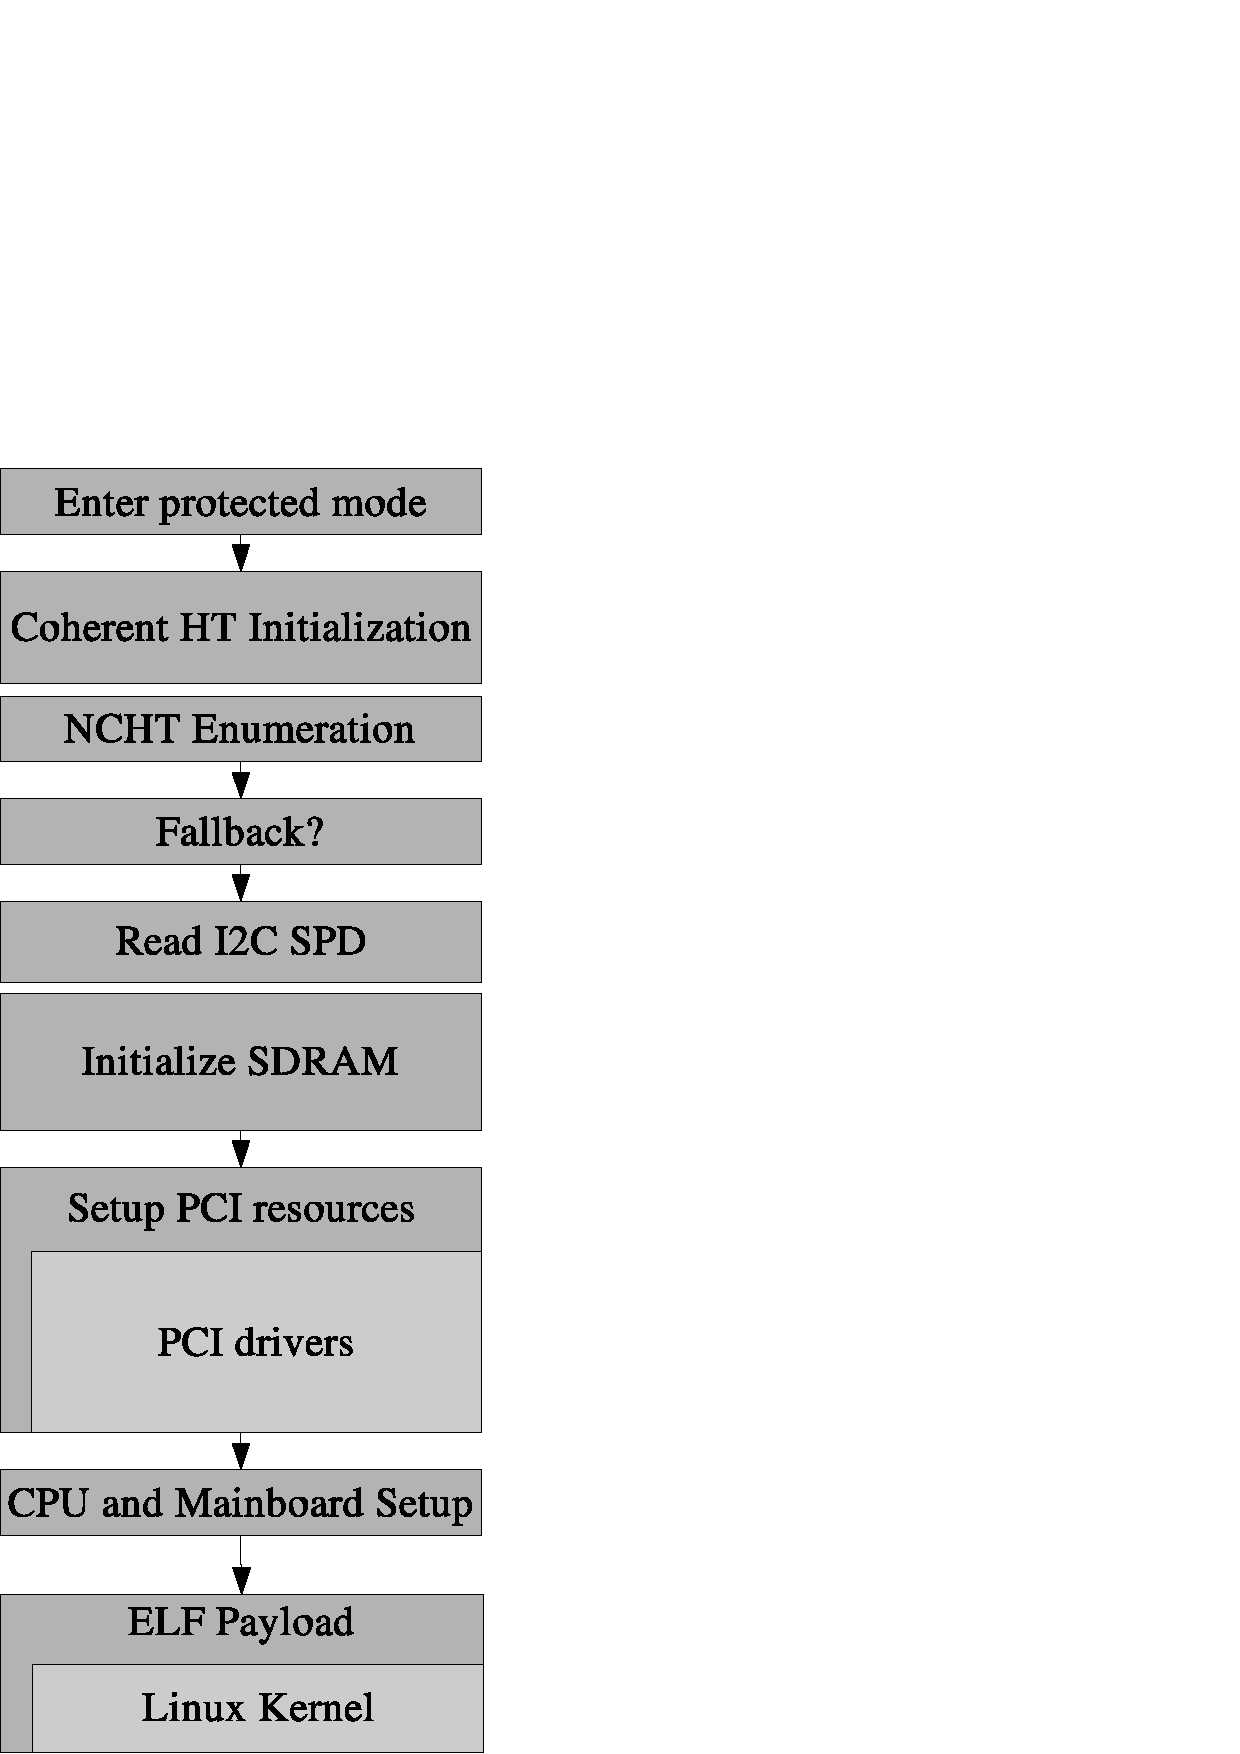
\includegraphics[scale=0.7]{codeflow.pdf}
\caption{coreboot rough Code Flow}
\label{fix:codeflow}
\end{figure}

\newpage

\subsection{Fallback mechanism}
coreboot provides a mechanism to pack two different coreboot builds
within one coreboot ROM image. Using the system CMOS memory coreboot
determines whether the last boot with a default image succeeded and
boots a failsafe image on failure. This allows insystem testing without
the risk to render the system unusable. See
\texttt{coreboot-v2/src/mainboard/arima/hdama/failover.c} for example
code. The fallback mechanism can be used with the \texttt{cmos\_util}.

\subsection{(Un) Supported Standards}
coreboot supports the following standards
\begin{itemize}
\item Multiprocessing Specification (MPSPEC) 1.4
\item IRQ Tables (PIRQ)
\item ACPI (initial support on AMD64)
\item Elf Booting
\end{itemize}
However, the following standards are not supported until now, and will
probably not be supported in future revisions:
\begin{itemize}
\item APM
\end{itemize}

\subsection{coreboot table}
coreboot stores information about the system in a data structure called
the coreboot table. This table can be read under Linux using the tool
nvramtool from the Lawrence Livermore National Laboratory.

Get more information about lxbios and the utility itself at
\url{http://www.llnl.gov/linux/lxbios/lxbios.html}

\subsection{ROMCC limitations}
ROMCC, part of the coreboot project, is a C compiler that translates to
completely rommable code. This means the resulting code does not need
any memory to work. This is one of the major improvements in coreboot
V2, since it allows almost all code to be written in C. DRAM
initialization can be factored and reused more easily among mainboards
and platforms.

Since no memory is available during this early initialization point,
romcc has to map all used variables in registers for the time being.
Same applies for their stack usage.  Generally the less registers are
used up by the algorithms, the better code can be factored, resulting in
a smaller object size. Since getting the best register usage is an NP
hard problem, some heuristics are used to get reasonable translation
time. If you run out of registers during compilation, try to refactor
your code.

\subsection{CMOS handling}
coreboot can use the mainboard's CMOS memory to store information
defined in a data structure called the CMOS table . This information
contains serial line speed, fallback boot control, output verbosity,
default boot device, ECC control, and more. It can be easily enhanced by
enhancing the CMOS table. This table, if present, is found at
\texttt{coreboot-v2/src/mainboard/$<$vendor$>$/$<$mainboard$>$/cmos.layout}.
It describes the available options, their possible values and their
position within the CMOS memory. The layout file looks as follows:
\begin{verbatim}
    # startbit length config configID    name
    [..]
           392      3      e        5    baud_rate
    [..]

    # configid value human readable description
      5        0     115200
      5        1      57600
      5        2      38400
      5        3      19200
      5        4       9600
      5        5       4800
      5        6       2400
      5        7       1200

\end{verbatim}

To change CMOS values from a running Linux system, use the
\texttt{cmos\_util}, provided by Linux Networks as part of the coreboot
utilities suite. Get it at
\textit{ftp://ftp.lnxi.com/pub/linuxbios/utilities/}

\subsection {Booting Payloads}
coreboot can load a payload binary from a Flash device or IDE. This
payload can be a boot loader, like FILO or Etherboot, a kernel image, or
any other static ELF binary.

To create a Linux kernel image, that is bootable in coreboot, you have
to use mkelfImage. The command line I used, looks like follows:

\begin{verbatim}
    objdir/sbin/mkelfImage t bzImagei386 kernel /boot/vmlinuz \
             commandline="console=ttyS0,115200 root=/dev/hda3" \
             initrd=/boot/initrd output vmlinuz.elf
\end{verbatim}


This will create the file \texttt{vmlinuz.elf} from a distribution
kernel, console redirected to the serial port and using an initial
ramdisk.

\subsection{Kernel on dhcp/tftp}

One possible scenario during testing is that you keep your kernel (or
any additional payload) on a different machine on the network. This can
quickly be done using a DHCP and TFTP server.

Use for example following \texttt{/etc/dhcpd.conf} (adapt to your
network):

\begin{verbatim}
    subnet 192.168.1.0 netmask 255.255.255.0 {
            range 192.168.1.0 192.168.1.31;
            option broadcastaddress 192.168.1.255;
    }

    ddnsupdatestyle adhoc;

    host hammer12 {
            hardware ethernet 00:04:76:EA:64:31;
            fixedaddress 192.168.1.24;
            filename "vmlinuz.elf";
    }
\end{verbatim}


Additionally you have to run a \texttt{tftp} server. You can start one
using \texttt{inetd}.  To do this, you have to remove the comment from
the following line in \texttt{/etc/inetd.conf}:

\begin{verbatim}
    tftp dgram udp wait root /usr/sbin/in.tftpd in.tftpd -s /tftpboot
\end{verbatim}

Then put your kernel image \texttt{vmlinuz.elf} in \texttt{/tftpboot} on
the \texttt{tftp} server.


\newpage

%
% 12. Advanced Device Initialization Mechanisms
%

\section{Advanced Device Initialization Mechanisms}

Like software, today's hardware is getting more and more complex. To
stay flexible many hardware vendors start breaking hardware
compatibility to old standards like VGA. Thus, VGA is still supported by
most cards, but emulation has to be enabled by the firmware for the
device to operate properly.  Also, many expansion cards are small
discrete systems that have to initialize attached ram, download
controller firmware and similar. Without this initialization, an
operating system can not take advantage of the hardware, so there needs
to be a way to address this issue. There are several alternatives:

\subsection{Native coreboot Support}

For some devices (ie Trident Cyberblade 3d) there is native coreboot
support This means there is a small driver bound to the PCI id of the
device that is called after PCI device ressources are allotted.

PROs:
 \begin{itemize}
 \item open source
 \item minimal driver
 \item early control
 \end{itemize}

CONs:
 \begin{itemize}
 \item need an additional driver
 \item viable for onboard devices only
 \item not flexible for pci cards
 \end{itemize}

\subsection{Using Native Linux Support}

A simple way of getting a whole lot of drivers available for coreboot
is to reuse Linux drivers by putting a Linux kernel to flash. This
works, because no drivers are needed to get the Linux kernel (as opposed
to store the kernel on a harddisk connected to isa/scsi/raid storage)

PROs:
 \begin{itemize}
 \item large number of open source drivers
 \end{itemize}

CONs:
 \begin{itemize}
 \item need Linux in Flash (BLOAT!)
 \item drivers expect devices to be initialized (LSI1020/1030)
 \item Linux only
 \item large flash needed (4MBit minimum, normal operations 8+ MBit)
 \end{itemize}


\subsection{Running X86 Option ROMs}

Especially SCSI/RAID controllers and graphics adapters come with a
special option rom. This option rom usually contains x86 binary code
that uses a legacy PCBIOS interface for device interaction. If this code
gets executed, the device becomes operable in Linux and other operating
systems.

PROs:
 \begin{itemize}
 \item really flexible
 \item no need for additional drivers on firmware layer
 \item large number of supported devices
 \end{itemize}

CONs:
 \begin{itemize}
 \item non-x86 platforms need complex emulation
 \item x86 platforms need legacy API
 \item outdated concept
 \end{itemize}


\subsection{Running Open Firmware Option ROMs}

Some PCI devices come with open firmware option roms. These devices are
normally found in computers from SUN, Apple or IBM. Open Firmware is a
instruction set architecture independent firmware standard that allows
device specific initialization using simple, small, but flexible
bytecode that runs with minimal footprint on all architectures that have
an Open Firmware implementation.

There is a free Open Firmware implementation available, called OpenBIOS,
that runs on top of coreboot. See www.openbios.org

PROs:
 \begin{itemize}
 \item architecture independence
 \item small footprint
 \item clean concept, less bugs
 \end{itemize}

CONs:
 \begin{itemize}
 \item only small number of devices come with OpenFirmware capable option roms
 \end{itemize}

%
% 13 image types
%

\section{Image types}
There used to be one image type for coreboot, as described above. Since this paper was written (2004) there have been many changes. First, the name
was changed to coreboot, for many reasons. Second, Cache As Ram support (CAR)
was added for many AMD CPUs, which both simplified and complicated things. Simplification came with the removal of romcc; complication came with the addition of new ways to build.

There are two big additions to the build process and, furthermore, more than two new CONFIG variables to control them.

\begin{itemize}
\item \begin{verbatim}CONFIG_USE_DCACHE_RAM\end{verbatim}

Set to \texttt{1} to use Cache As Ram (CAR). Defaults to \texttt{0}

\end{itemize}

Before going over the new image types, derived from v3, we will quickly review the standard v2 image types. We are hoping this review will
aid comprehension.

A coreboot rom file consists of one or more \textit{images}. All images consist of a part that runs in ROM, and a part that runs in RAM. The RAM can be in  compressed form and is decompressed when needed by the ROM code. The main function of the ROM code is to get memory working. Both ROM and RAM consist of a very small amount of assembly code and mostly C code.

\subsection{romcc images (from emulation/qemu)}
ROMCC images are so-called because C code for the ROM part is compiled with romcc. romcc is an optimizing C compiler which compiles one, and only
one file; to get more than one file, one must include the C code via include statements. The main ROM code .c file is usually called auto.c.
\subsubsection{How it is built}
Romcc compiles auto.c to produce auto.inc. auto.inc is included in the main crt0.S, which is then preprocessed to produce crt0.s. The inclusion of files into crt0.S is controlled by the CONFIG\_CRT0\_INCLUDES variable. crt0.s is then assembled.

File for the ram part are compiled in a conventional manner.

The final step is linking. The use of named sections is used very heavily in coreboot to control where different bits of code go. The reset vector must go in the top 16 bytes. The start portion of the ROM code must go in the top 64K bytes, since most chipsets only enable this much ROM at startup time. Here is a quick look at a typical image:
\begin{verbatim}
  [Nr] Name              Type            Addr     Off    Size   ES Flg Lk Inf Al
  [ 0]                   NULL            00000000 000000 000000 00      0   0  0
  [ 1] .ram              PROGBITS        ffff0000 001000 005893 00  WA  0   0  1
  [ 2] .rom              PROGBITS        ffff5893 006893 00029d 00  AX  0   0 16
  [ 3] .reset            PROGBITS        fffffff0 006ff0 000010 00   A  0   0  1
  [ 4] .id               PROGBITS        ffffffd1 006fd1 00001f 00   A  0   0  1
  [ 5] .shstrtab         STRTAB          00000000 007000 000030 00      0   0  1
  [ 6] .symtab           SYMTAB          00000000 007170 000c30 10      7  37  4
  [ 7] .strtab           STRTAB          00000000 007da0 000bfd 00      0   0  1
\end{verbatim}

The only sections that get loaded into a ROM are the Allocated ones. We can see the .ram, .rom, .reset and .id sections.
\subsubsection{layout}
As we mentioned, the ROM file consists of multiple images. In the basic file, there are two full coreboot rom images. The build sequence for each is the same, and in fact the ldscript.ld files are almost identical. The only difference is in a few makefile variables, generated by the config tool.

\begin{itemize}
\item CONFIG\_PAYLOAD\_SIZE. Each image may have a different payload size.
\item CONFIG\_ROMBASE Each image must have a different base in rom.
\item CONFIG\_RESET Unclear what this is used for.
\item CONFIG\_EXCEPTION\_VECTORS where an optional IDT might go.
\item CONFIG\_USE\_OPTION\_TABLE if set, an option table section will be linked in.
\item CONFIG\_ROM\_PAYLOAD\_START This is the soon-to-be-deprecated way of locating a payload. cbfs eliminates this.
\item CONFIG\_USE\_FALLBACK\_IMAGE Whether this is a fallback or normal image
\item CONFIG\_ROM\_SECTION\_SIZE Essentially, the payload size. Soon to be deprecated.
\item CONFIG\_ROM\_IMAGE\_SIZE Size of this image (i.e. fallback or normal image)
\item CONFIG\_ROM\_SIZE Total size of the ROM
\item CONFIG\_XIP\_RAM\_BASE The start of eXecute In Place code. XIP allows for not copying code to ram, but just running it from ROM.
\end{itemize}

Each image (normal or fallback) is built completely independently and does not get linked to the other. They are assembled into one ROM image by the (soon to be deprecated) buildrom tool, or by the cbfs tool.

\subsubsection{boot sequence}
We boot and start at fffffff0. We then jump to the entry point at \_start.  \_start does some machine init and an lgdt and jumps to \_\_protected\_start, at which point we are in protected mode. The code does a bit more machine setup and then starts executing the romcc code.

If fallback has been built in, some setup needs to be done. On some machines, it is extensive. Full rom decoding must be enabled. This may in turn require additional PCI setup to enable decoding to be enabled (!). To decided which image to use, hardware registers (cold boot on the Opteron) or CMOS are checked. Finally, once the image to use has been decided, a jmp is performed, viz:
\begin{verbatim}
        /* This is the primary cpu how should I boot? */
        else if (do_normal_boot()) {
                goto normal_image;
        }
        else {
                goto fallback_image;
        }
 normal_image:
        __asm__ volatile ("jmp __normal_image"
                : /* outputs */
                : "a" (bist), "b" (cpu_init_detectedx) /* inputs */
                );

 fallback_image:
#if CONFIG_HAVE_FAILOVER_BOOT==1
        __asm__ volatile ("jmp __fallback_image"
                : /* outputs */
                : "a" (bist), "b" (cpu_init_detectedx) /* inputs */
                )
#endif
        ;
\end{verbatim}
How does the fallback image get the symbol for normal entry? Via magic in the ldscript.ld -- remember, the images are not linked to each other.
Finally, we can see this in the Config.lb for most mainboards:
\begin{verbatim}
if CONFIG_USE_FALLBACK_IMAGE
        mainboardinit cpu/x86/16bit/reset16.inc
        ldscript /cpu/x86/16bit/reset16.lds
else
        mainboardinit cpu/x86/32bit/reset32.inc
        ldscript /cpu/x86/32bit/reset32.lds
end
\end{verbatim}
What does this mean? the non-fallback image has a 32-bit entry point; fallback has a 16-bit entry point. The reason for this is that some code from fallback always runs, so as to pick fallback or normal; but the normal is always called from 32-bit code.
\subsection{car images (from lippert/roadrunner-lx)}
CAR images in their simplest form are modified romcc images. The file is usually cache\_as\_ram\_auto.c. C inclusion is still used. The main difference is in the build sequence. The compiler command line is a very slight changed: instead of using romcc to generate an auto.inc include file, gcc us used. Then, two perl scripts are used to rename the .text and .data sections to .rom.text and .rom.data respectively.
\subsubsection{How it is built}
The build is almost identical to the romcc build. Since the auto.inc file exists, it can be included as before. The crt0\_includes.h file has one addition: a file that enables CAR, in this case it is \textit{src/cpu/amd/model\_lx/cache\_as\_ram.inc}.
\subsubsection{layout}
No significant change from romcc code.
\subsubsection{boot sequence}
No significant change from romcc code, except that the CAR code has to set up a stack.

\subsection{car + CONFIG\_USE\_INIT images (new emulation/qemu}
This type of image makes more use of the C compiler. In this type of image, in fact,
seperate compilation is possible but is not always used. Oddly enough, this option is only used in PPC boards. That said, we need to move to this way of building. Including C code is poor style.
\subsubsection{How it is built}
There is a make variable, INIT-OBJECTS, that for all our other targets is empty. In this type of build, INIT-OBJECTS is a list of C files that are created from the config tool initobject command. Again, with INIT-OBJECTS we can finally stop including .c files and go with seperate compilation.
\subsubsection{layout}
No significant change from romcc code.
\subsubsection{boot sequence}
No significant change from romcc code, except that the CAR code has to set up a stack.

\subsubsection{layout}
No significant change from romcc code.
\subsubsection{boot sequence}
No significant change from romcc code, except that the CAR code has to set up a stack.
\subsection{failover}
Failover is the newest way to lay out a ROM. The choice of which image to run is removed from the fallback image and moved into a small, standalone piece of code. The code is simple enough to show here:
\begin{verbatim}
static unsigned long main(unsigned long bist)
{
	if (do_normal_boot())
		goto normal_image;
	else
		goto fallback_image;

normal_image:
	__asm__ __volatile__("jmp __normal_image" : : "a" (bist) : );

cpu_reset:
	__asm__ __volatile__("jmp __cpu_reset" : : "a" (bist) : );

fallback_image:
	return bist;
}

\end{verbatim}
Some motherboards have a more complex bus structure (e.g. Opteron). In those cases, the failover can be more complex, as it requires some hardware initialization to work correctly. As of this writing (April 2009), these boards have their own failover:
\begin{quote}
./src/mainboard/iei/nova4899r/failover.c
./src/mainboard/emulation/qemu-x86/failover.c
./src/mainboard/supermicro/x6dhr\_ig/failover.c
./src/mainboard/supermicro/x6dai\_g/failover.c
./src/mainboard/supermicro/x6dhe\_g2/failover.c
./src/mainboard/supermicro/x6dhr\_ig2/failover.c
./src/mainboard/supermicro/x6dhe\_g/failover.c
./src/mainboard/dell/s1850/failover.c
./src/mainboard/intel/xe7501devkit/failover.c
./src/mainboard/intel/jarrell/failover.c
./src/mainboard/olpc/btest/failover.c
./src/mainboard/olpc/rev\_a/failover.c
./src/mainboard/via/epia-m/failover.c
\end{quote}
Here is one of the more complicated ones:
\begin{verbatim}
static unsigned long main(unsigned long bist)
{
        /* Did just the cpu reset? */
        if (memory_initialized()) {
                if (last_boot_normal()) {
                        goto normal_image;
                } else {
                        goto cpu_reset;
                }
        }

        /* This is the primary cpu how should I boot? */
        else if (do_normal_boot()) {
                goto normal_image;
        }
        else {
                goto fallback_image;
        }
 normal_image:
        asm volatile ("jmp __normal_image"
                : /* outputs */
                : "a" (bist) /* inputs */
                : /* clobbers */
                );
 cpu_reset:
        asm volatile ("jmp __cpu_reset"
                : /* outputs */
                : "a"(bist) /* inputs */
                : /* clobbers */
                );
 fallback_image:
        return bist;
}

\end{verbatim}
They're not that different, in fact. So why are there different copies all over the tree? Simple: code inclusion. Most of the failover.c are different because they include different bits of code. Here is a key reason for killing C code inclusion in the tree.
\subsubsection{How it is built}
There two additional config variables:
\begin{itemize}
\item HAVE\_FAILOVER\_IMAGE Has to be defined when certain files are included.
\item USE\_FAILOVER\_IMAGE Enables the use of the failover image
\end{itemize}
Confusingly enough, almost all the uses of these two variables are either nested or both required to be set, e.g.
The fallback and normal builds are the same. The target config has a new clause that looks like this:
\begin{verbatim}
romimage "failover"
        option CONFIG_USE_FAILOVER_IMAGE=1
        option CONFIG_USE_FALLBACK_IMAGE=0
        option CONFIG_ROM_IMAGE_SIZE=CONFIG_FAILOVER_SIZE
        option CONFIG_XIP_ROM_SIZE=CONFIG_FAILOVER_SIZE
        option COREBOOT_EXTRA_VERSION="\$(shell cat ../../VERSION)\_Failover"
end
\end{verbatim}
This new section uses some constructs not yet discussed in detail. XIP\_ROM\_SIZE just refers to the
fact that the failover code is eXecute In Place, i.e. not copied to RAM. Of course, the ROM part of normal/fallback is as well, so the usage of XIP here is somewhat confusing. Finally, the USE\_FAILOVER\_IMAGE variable is set, which changes code compilation in a few places. If we just consider non-mainbard files, there are:
\begin{verbatim}
src/cpu/amd/car/cache_as_ram.inc
src/arch/i386/Config.lb
\end{verbatim}
For the cache\_as\_ram.inc file, the changes relate to the fact that failover code sets up CAR, so that fallback code need not.

For the Config.lb, several aspects of build change.
When USE\_FAILOVER\_IMAGE, entry into both normal and fallback bios images is via a 32-bit entry point (when not defined, entry into fallback is a 16-entry point at the power-on reset vector).
\subsubsection{layout}
Failover.c becomes the new bootblock at the top of memory. It calls either normal or fallback. The address of normal and fallback is determined by ldscript magic.
\subsubsection{boot sequence}
failover.c tests a few variables and the calls the normal or fallback payload depending on those variables; usually they are CMOS settings.
\subsection{Proposed new image forat}
The new image format will use seperate compilation -- no C code included! -- on all files.

The new design has a few key goals:
\begin{itemize}
\item Always use a bootblock (currently called failover).
The name failover.c, being utterly obscure, will not be used; instead, we will name the file bootblock.c. Instead of having a different copy for each mainboard, we can have just one copy.
\item Always use seperate compilation
\item Always use printk etc. in the ROM code
\item (longer term) from the bootblock, always use cbfs to locate the normal/fallback etc. code. This code will be XIP.
\end{itemize}

\subsubsection{How it is built}
For now, since we are still using the config tool, we'll need a new command: bootblockobject, which creates a list of files to be included in the bootblock.   Not a lot else will have to change. We are going to move to using the v3 CAR code assembly code (one or two files at most, instead of many) and, instead of the thicket of little ldscript files, one ldscript file. This strategy is subject to modification as events dictate.
\subsubsection{layout}
Almost the same, for now, as the current failover code.
\subsubsection{boot sequence}
%
% 14 Glossary
%

\section{Glossary}
\begin{itemize}
\item payload

coreboot only cares about low level machine initialization, but also has
very simple mechanisms to boot a file either from FLASHROM or IDE. That
file, possibly a Linux Kernel, a boot loader or Etherboot, are called
payload, since it is the first software executed that does not cope with
pure initialization.

\item flash device

Flash devices are commonly used in all different computers since unlike
ROMs they can be electronically erased and reprogrammed.
\end{itemize}

\newpage

%
% 14 Bibliography
%

\section{Bibliography}
\subsection{Additional Papers on coreboot}

\begin{itemize}
 \item
 \textit{\url{http://www.coreboot.org/Documentation}}
 \item
 \textit{\url{http://www.lysator.liu.se/upplysning/fa/linuxbios.pdf}}
 \item
 \textit{\url{http://portal.acm.org/citation.cfm?id=512627}}
\end{itemize}

\subsection {Links}

\begin{itemize}
 \item Etherboot: \textit{\url{http://www.etherboot.org/}}
 \item Filo: \textit{\url{http://www.coreboot.org/FILO}}
 \item OpenBIOS: \textit{\url{http://www.openbios.org/}}
\end{itemize}

\end{document}
